% --------------------------------------------------------------------------------

\begin{exercise}[Exercise 5.9]

Modify the algorithm for first-visit MC policy evaluation (Section 5.1)
to use the incremental implementation for sample averages described in
Section 2.4.

\begin{figure}[H]
    \centering
    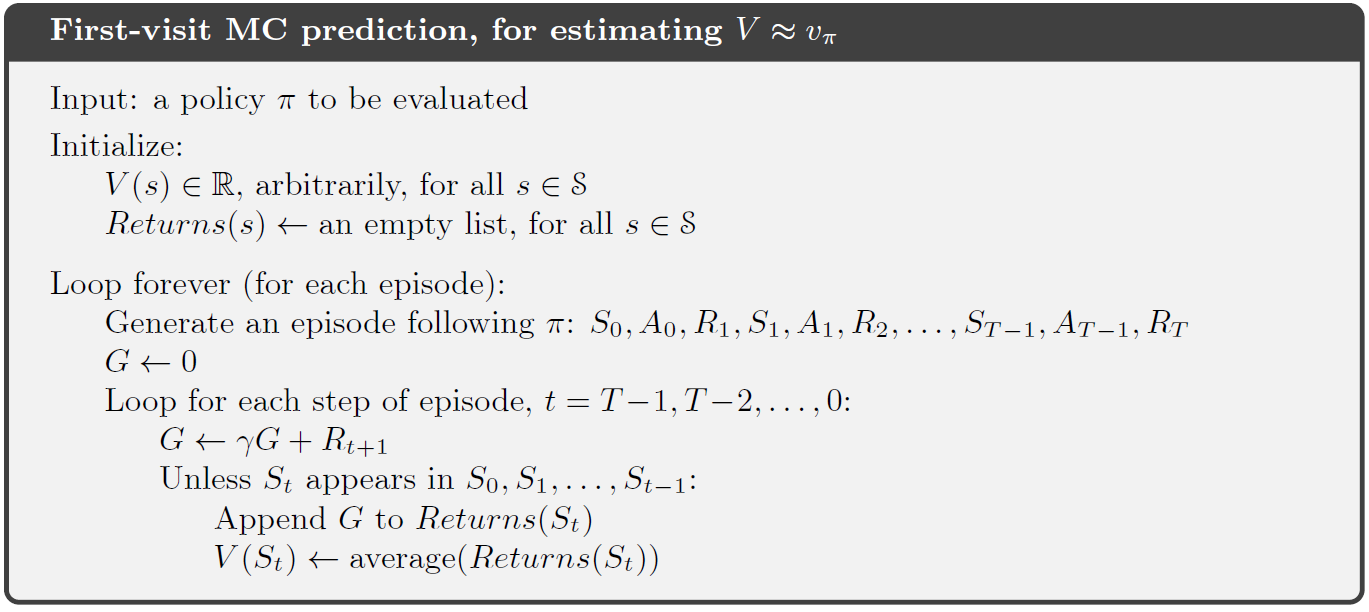
\includegraphics[width = 0.8 \textwidth]{alg_4.2.png}
\end{figure}
  
\end{exercise}
  
% --------------------------------------------------------------------------------
  
\begin{solution}

\phantom{}
  
\begin{algorithm}
    \caption{First-visit MC prediction, for estimating $V \approx v_\pi$}
    \hspace*{\algorithmicindent} \textbf{Input:} a policy $\pi$ to be evaluated
    \begin{algorithmic}[1]
      \State Initialize $V(s) \in \R$ arbitrarily for all $s \in \mathcal{S}$
      \State Initialize Counter$(s) \leftarrow 0$ for all $s \in \mathcal{S}$
      \While{True (for each episode)}
        \State Generate an episode following $\pi: S_0,A_0,R_1,\dots,S_{T-1},A_{T-1},R_T$
        \State $G \leftarrow 0$
        \For{$t = T-1,\dots,0$}
        \State $G \leftarrow \gamma G + R_{t+1}$
        \If{NOT $S_t$ appears in $S_0,\dots,S_{t-1}$}
        \State Counter$(S_t) \leftarrow \text{Counter}(S_t) + 1$
        \State $V(S_t) \leftarrow V(S_t) +  \frac{1}{\text{Counter}(S_t)}[G - V(S_t)]$
        \EndIf
        \EndFor
      \EndWhile
    \end{algorithmic}
\end{algorithm}
  
\end{solution}
  
% --------------------------------------------------------------------------------
  